\documentclass[11pt]{article}
\usepackage{geometry}                
\geometry{letterpaper}                   

\usepackage{graphicx}
\usepackage{amssymb}
\usepackage{epstopdf}
\usepackage{natbib}
\usepackage{amssymb, amsmath}
\DeclareGraphicsRule{.tif}{png}{.png}{`convert #1 `dirname #1`/`basename #1 .tif`.png}

%\title{Title}
%\author{Name 1, Name 2}
%\date{date} 

\begin{document}



\thispagestyle{empty}

\begin{center}

\includegraphics[width=5cm]{ETHlogo.eps}

\bigskip


\bigskip


\bigskip


\LARGE{ 	Lecture with Computer Exercises:\\ }
\LARGE{ Modelling and Simulating Social Systems with MATLAB\\}

\bigskip

\bigskip

\small{Project Report}\\

\bigskip

\bigskip

\bigskip

\bigskip


\begin{tabular}{|c|}
\hline
\\
\textbf{\LARGE{Insert Title Here}}\\
\textbf{\LARGE{...}}\\
\\
\hline
\end{tabular}
\bigskip

\bigskip

\bigskip

\LARGE{Name 1 \& Name 2}



\bigskip

\bigskip

\bigskip

\bigskip

\bigskip

\bigskip

\bigskip

\bigskip

Zurich\\
May 2008\\

\end{center}



\newpage

%%%%%%%%%%%%%%%%%%%%%%%%%%%%%%%%%%%%%%%%%%%%%%%%%

\newpage
\section*{Agreement for free-download}
\bigskip


\bigskip


\large We hereby agree to make our source code for this project freely available for download from the web pages of the SOMS chair. Furthermore, we assure that all source code is written by ourselves and is not violating any copyright restrictions.
Several external packages are used that are freely available at Matlab FileExchange under a BSU license. 
\begin{center}

\bigskip


\bigskip


\begin{tabular}{@{}p{3.3cm}@{}p{6cm}@{}@{}p{6cm}@{}}
\begin{minipage}{3cm}

\end{minipage}
&
\begin{minipage}{6cm}
\vspace{2mm} \large Fabio Crameri

 %\vspace{\baselineskip}

\end{minipage}
&
\begin{minipage}{6cm}

\vspace{2mm} \large Marcel Thielmann

\end{minipage}
\end{tabular}


\end{center}
\newpage

%%%%%%%%%%%%%%%%%%%%%%%%%%%%%%%%%%%%%%%



% IMPORTANT
% you MUST include the ETH declaration of originality here; it is available for download on the course website or at http://www.ethz.ch/faculty/exams/plagiarism/index_EN; it can be printed as pdf and should be filled out in handwriting


%%%%%%%%%% Table of content %%%%%%%%%%%%%%%%%

\tableofcontents

\newpage

%%%%%%%%%%%%%%%%%%%%%%%%%%%%%%%%%%%%%%%



\section{Abstract}

Hei M\"ase, we should first define what we mean by social and physical forces. I'm not sure if there is something like social forces between an agent and a wall. I mean normally there is not...

Hei F�bu, in dem Helbing paper gibts definitiv social forces zwischen Wand und den agents. Irgendwie soll das ausdr�cken, dass die agents nicht so nah an der Wand laufen wollen. Wir k�nnen aber auch argumentieren, dass diese Kr�fte in ner Paniksituation ziemlich wurscht sind.

I don't know how to make bold characters

\section{Individual contributions}
Marcel: 376 bugs
Fabio: 376 bugfixes

\section{Introduction and Motivations}

\section{Description of the Model}

\subsection{Agent}
\subsubsection{Psychological forces}

\subsubsection{Physical forces}


\subsection{Walls}

\subsubsection{Psychological forces}

The psychological repulsive force defined here for the walls/buildings can be written in mathematical terms as

\begin{equation}
	{f_{iWS}} = \left\{ {{A_i}\exp \left[ {\frac{{\left( {{r_i} - {d_{iW}}} \right)}}{{{B_i}}}} \right]} \right\}{n_{iW}} ,
	\label{eq:fiWS}
\end{equation}

where $A_i$ and $B_i$ are constants, $n_{iW}$ is the normalized vector pointing from the pedestrian to the wall, $d_{iW}$ is the distance in between and $r_i$ is the size (i.e. radius) of the pedestrian (Helbing et al., 2000).

\subsubsection{Physical forces}

The physical wall forces can be divided into a normal force and a tangential force acting from the wall and written as

\begin{equation}
	{f_{iWPn}} = \left\{ {kg\left( {{r_i} - {d_{iW}}} \right)} \right\}{n_{iW}}
	\label{eq:fiWPn}
\end{equation}

and

\begin{equation}
	{f_{iWPt}} = \left\{ {\kappa g\left( {{r_i} - {d_{iW}}} \right)\left( {{v_i} \cdot {t_{iW}}} \right)} \right\}{t_{iW}} ,
	\label{eq:fiWPt}
\end{equation}

respectively. Here, the function $g$ is zero if the pedestrian does not touch the wall, $k$ and $\kappa$ are large constants and $(v_i \cdot t_{iW})$ is the tangential velocity difference.

The total repulsive force from the architecture can then be written as

\begin{equation}
	{f_{iW}} = {f_{iWS}} + {f_{iWPn}} - {f_{iWPt}} .
	\label{eq:fiW}
\end{equation}



\subsection{Exits}
\label{sec:Exits1}

In our model, the sole attractive force is the exit force. As for the social forces, it is rather a psychological force representing the will of each agent to reach the exit. In this work, we chose the value of the exit force to be proportional to the sum of the other psychological forces (in our code, one can choose a proportionality constant to adjust the exit force). To determine the direction of the exit force, we used two different approaches: i) the agent is drawn directly towards the exit, regardless of any obstacles in between him and an exit, and ii) the agent decides on its walking direction based on the estimate of the time it needs to reach the exit.

While i) is relatively straightforward to implement, there are several crucial drawbacks to this method: First, it does not reflect at all the decision process of a human agent, since obstacles between the agent and the exit are always taken into account. Second, 

\subsubsection{Shortest path formulation}

Finding the shortest path between two points is a mathematical problem that has received much attention since it's solution can be used in a huge number of applications. One of the earliest solutions to this problem was presented by Dykstra (reference). Shebian (right name? reference?) presented a fast and efficient method to solve a certain class of shortest path problems, which  is called the Fast marching method. It is a special case of level set methods and solve the Eikonal equation (equation?). 

This equation describes the We can essentially apply this algorithm to our problem

In a more sophisticated version of the code, we make use of a fast marching algorithm that takes into account walls as being regions with a low velocity. We compute the shortest path


\subsection{Flood}

\subsection{Topography}

\subsection{Walking speed}



\section{Implementation}

This section is meant to both give an overview of the methods used in this code as well as to provide a documentation of the code. Therefore, some details are mentioned here that might not be crucial for any code that simulates pedestrian dynamics, but are needed in our implementation. 

\subsection{Initialization of Buildings and Agents}

\subsection{Agents}

\subsubsection{Agent forces}


\subsection{Architecture}

\subsubsection{Repulsive walls}

Eq.~\eqref{eq:fiWS} can be rewritten as

\begin{equation}
	{f_{iWS}} = \left\{ {{A_i}\left( {\exp \left[ {\frac{{ - {d_{iW}}}}{{{B_i}}}} \right] \cdot \exp \left[ {\frac{{{r_i}}}{{{B_i}}}} \right]} \right)} \right\}{n_{iW}}
	\label{eq:fiWS2}
\end{equation}

\subsubsection{Exit forces}

In this section, we show two approaches to tackle the problem of the psychological exit force. Using small and rather simple models, we show the differences that arise from the different implementations. We then choose one of

\subsection{Walking speed}

\subsection{Flooding}



\section{Simulation Results and Discussion}

\subsection{Simple evacuation bottleneck: One exit}

\subsubsection{Direct exit force}

\begin{figure}
	\begin{center}
	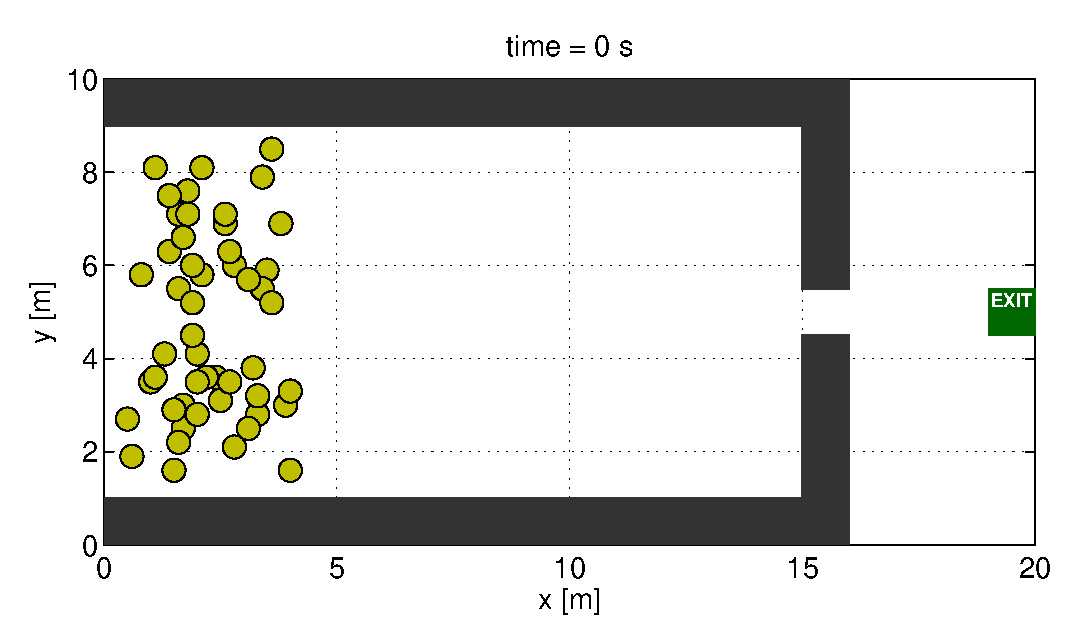
\includegraphics[width=0.7\textwidth]
	{figures/Model1_direct_1_000000.eps}
	\qquad
	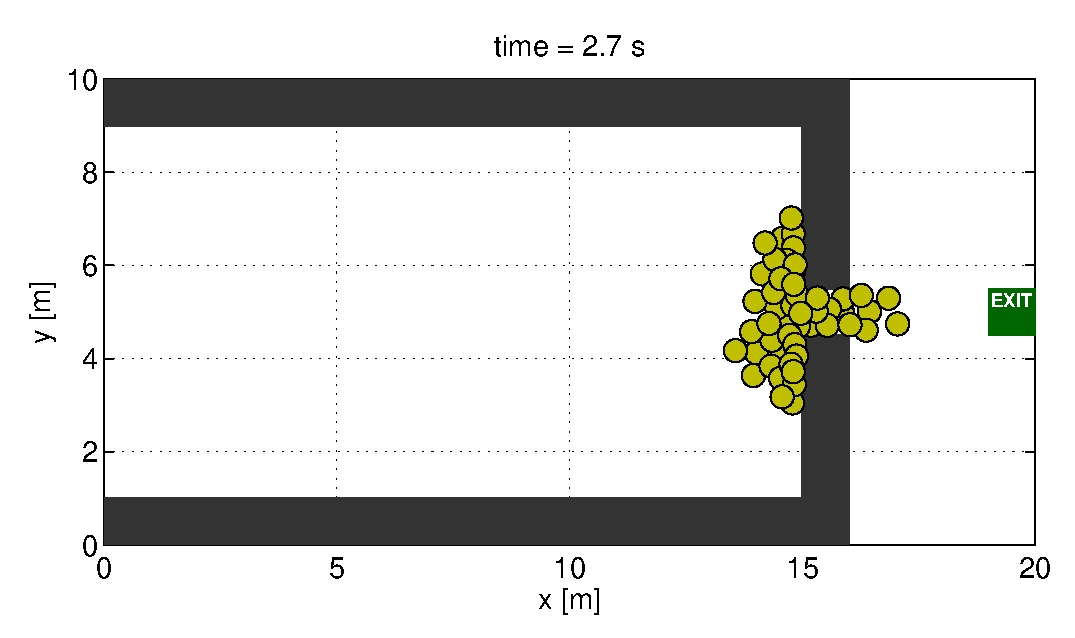
\includegraphics[width=0.7\textwidth]
	{figures/Model1_direct_1_000270.eps}
	\qquad
	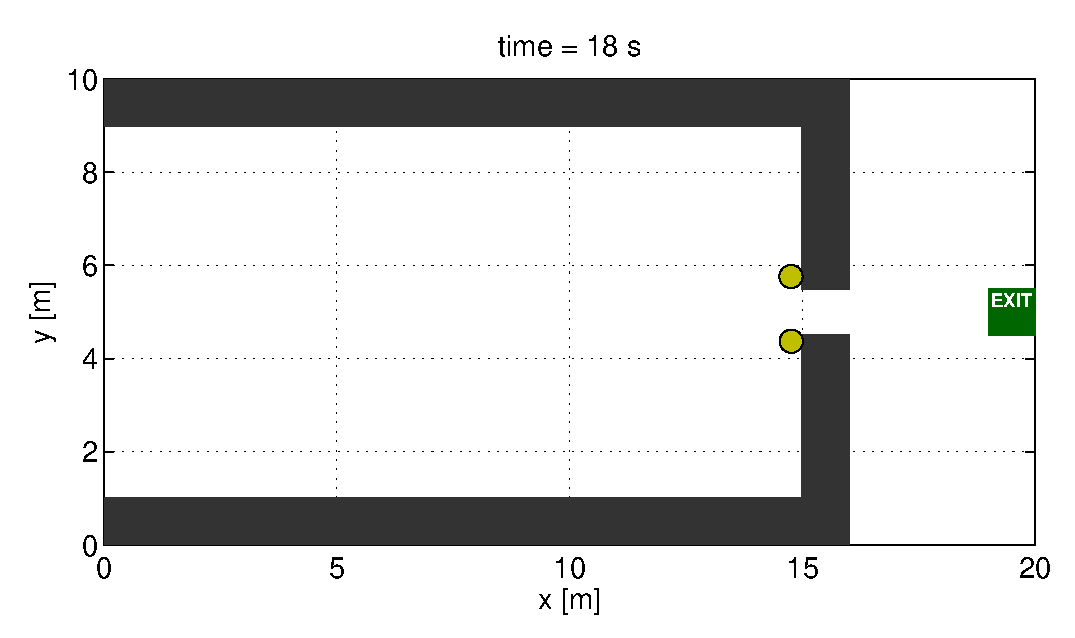
\includegraphics[width=0.7\textwidth]
	{figures/Model1_direct_1_001800.eps}
	\caption{Simple starting model for a room evacuation through a bottleneck. (a) Initial setup, (b) agents arriving at the bottleneck and accumulating in behind and (c) agents blocking each other of exiting at the end of the simulation.}
	\label{fig:simple1}
	\end{center}
\end{figure}

The simplest version of our code has one exit (Fig.~\ref{fig:simple1}). The attractive force on the agents is defined to be linear towards the exit, thereby neglecting obstacles in between. The agents will not move towards an opening in an obstacle but toward the exit itself. Moreover, this formulation inhibits the agents of running around a bigger obstacle. This is a strong simplification but suitable to test the code. The behavior of the agents towards the repulsive walls and towards each other is satisfactory.

A first case ({\it Model1\_linear\_1}) is shown in Fig.~\ref{fig:simple1}. The model setup consists of a $15\times9$ m room that is bounded by repulsive walls. A $1\times1$ m door is the only exit thereof and leads to the attractive main exit of the model. The agents are initially placed randomly in an $3.5\times7$ m area in the left hand side of the domain (Fig.~\ref{fig:simple1}b). The model is not satisfactory, because at the late stage of evacuation there are two agents opposite of each other preventing them to exit the room (Fig.~\ref{fig:simple1}c). The counter parting psychologic social forces cancel all other forces out and therefore both agents remain at their position.

\begin{figure}
	\begin{center}
	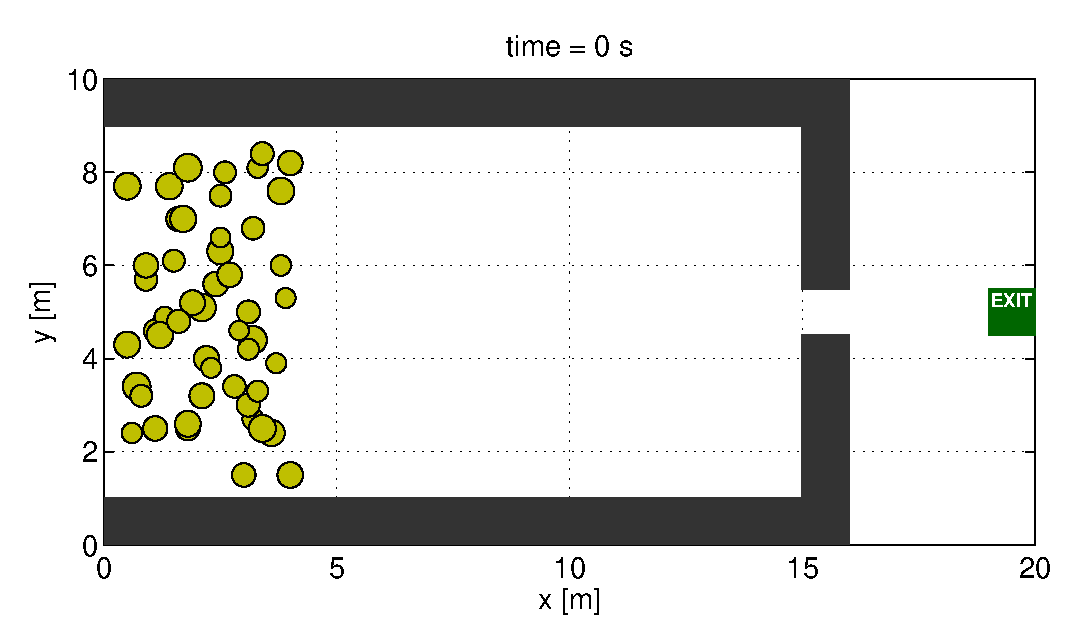
\includegraphics[width=0.7\textwidth]
	{figures/Model1_direct_2_000000.eps}
	\qquad
	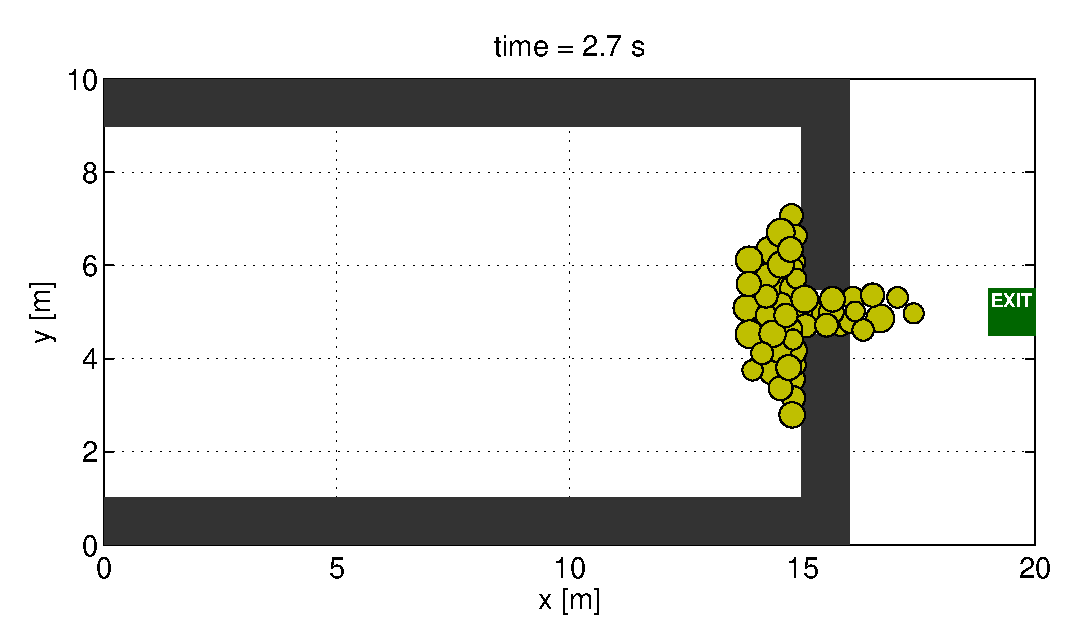
\includegraphics[width=0.7\textwidth]
	{figures/Model1_direct_2_000270.eps}
	\qquad
	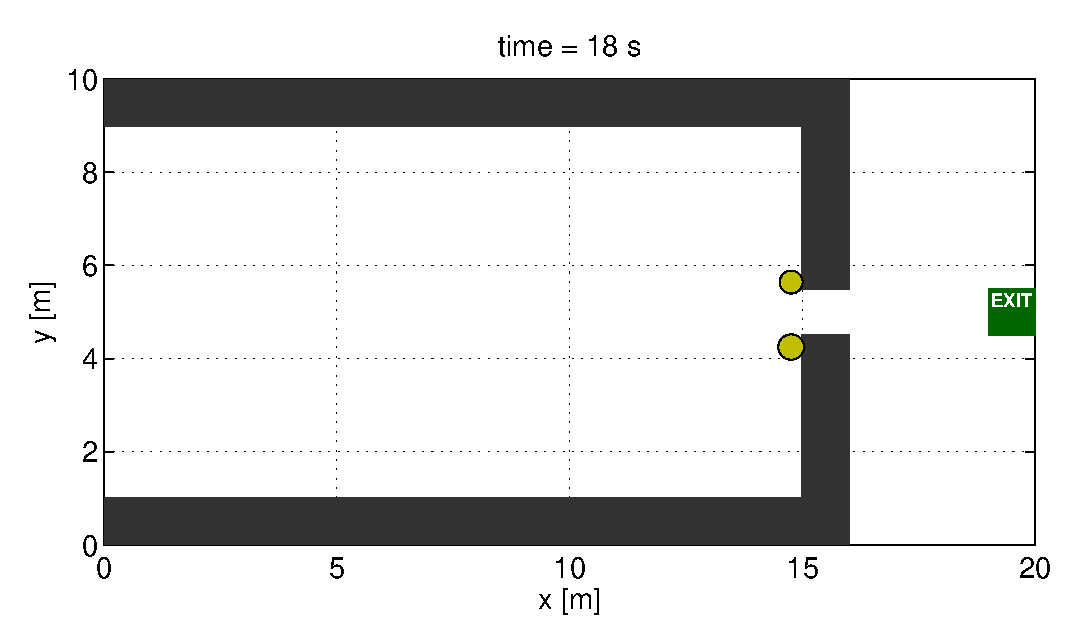
\includegraphics[width=0.7\textwidth]
	{figures/Model1_direct_2_001800.eps}
	\caption{Model including perturbations for a room evacuation through a bottleneck. (a) Initial setup, (b) agents arriving at the bottleneck and accumulating in behind and (c) agents blocking each other of exiting at the end of the simulation.}
	\label{fig:simple2}
	\end{center}
\end{figure}

In order to introduce some noise into an otherwise perfect model we added several perturbations ({\it Model1\_linear\_2}). The psychologic social force between the agents is perturbed by a random small value in the order of $\pm 0.05$ N. Another complexity is added by characterizing the different agents. Accounting for different appetite and/or stomach behavior, their mass is randomly chosen with a perturbation of $\pm 10$ kg. A bigger radius is subsequently needed for fulfilling mass conservation. Therefore the agent's radius is randomly perturbed by $\pm 0.05$ m. The results of these adjustments are shown in Fig.~\ref{fig:simple2}.

Still the last two pedestrians are disabled of leaving the room because of the counteracting forces they exert on each other. This shows, that the "perfectness" of the model was not the main problem of this occurrence. The main cause of it might be found in the way the attractive exit force is described. The agents are pulled with the exit force directly towards the position of the exit, neglecting possible obstacles in between. Hence, in the case of the two blocked pedestrians, the main force is directed perpendicular to the wall instead of tangential to the wall towards the wall door. The force in this direction is very small and can thus easily be overweighted by the repulsive social force of the opposite agent. The agent is kept at his current position.

A solution of this problem therefore might be found in a different description of the attractive exit force by e.g. a fastest path formulation.


\subsubsection{Shortest path formulation}

The shortest path formulation as described in Section~\ref{sec:Exits1} can improve the nature-like behavior of the model dramatically. A new setup is chosen to illustrate this and shown in Fig.~\ref{fig:simple3} and~\ref{fig:simple4}.

\begin{figure}
	\begin{center}
	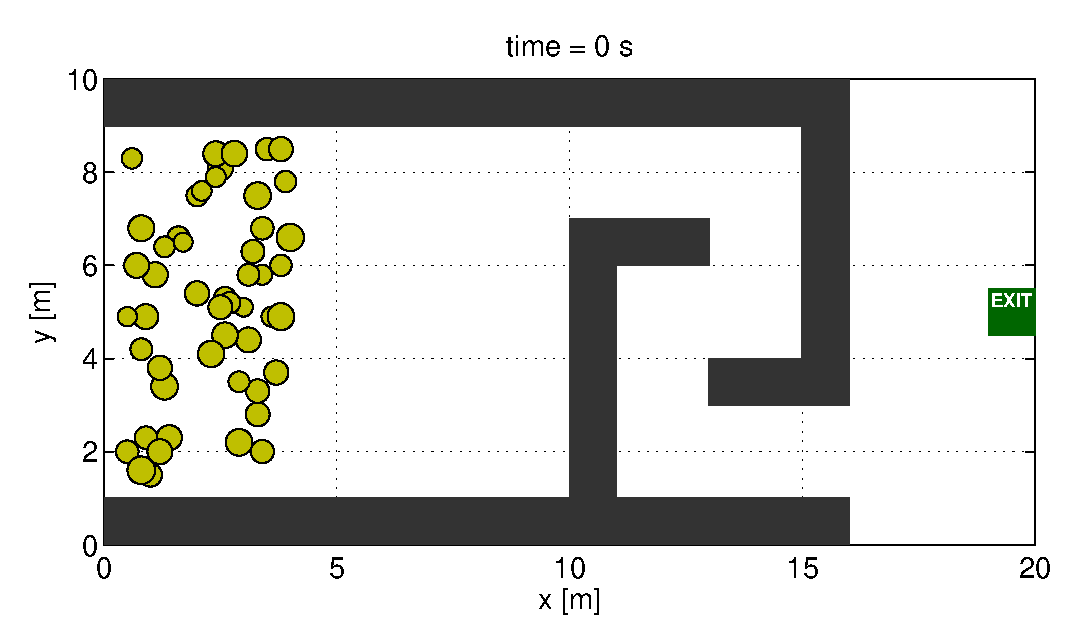
\includegraphics[width=0.7\textwidth]
	{figures/Model2_direct_1_000000.eps}
	\qquad
	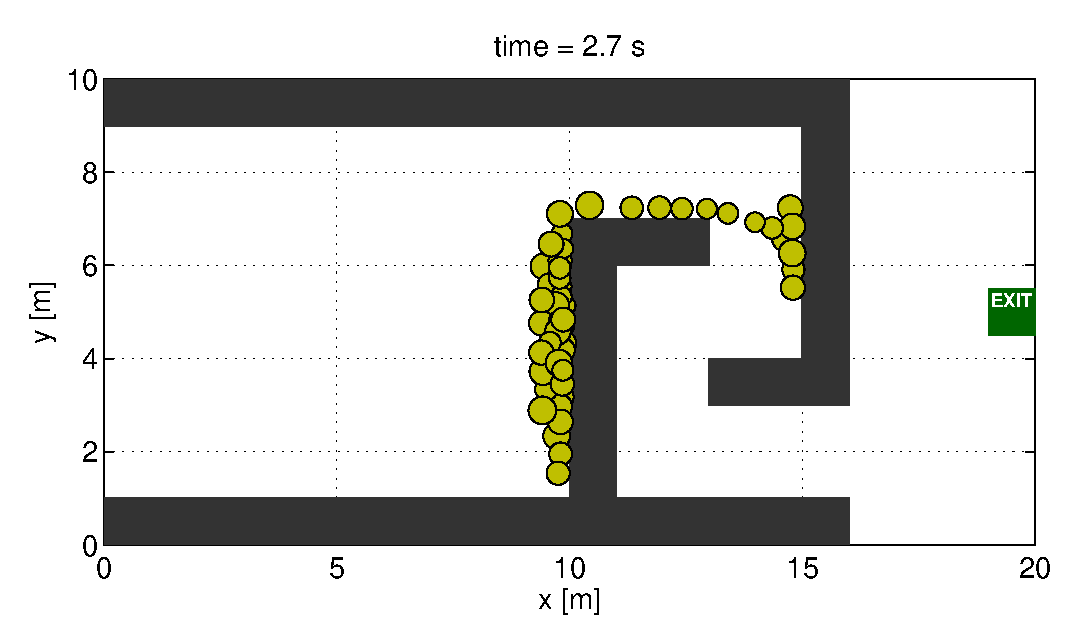
\includegraphics[width=0.7\textwidth]
	{figures/Model2_direct_1_000270.eps}
	\qquad
	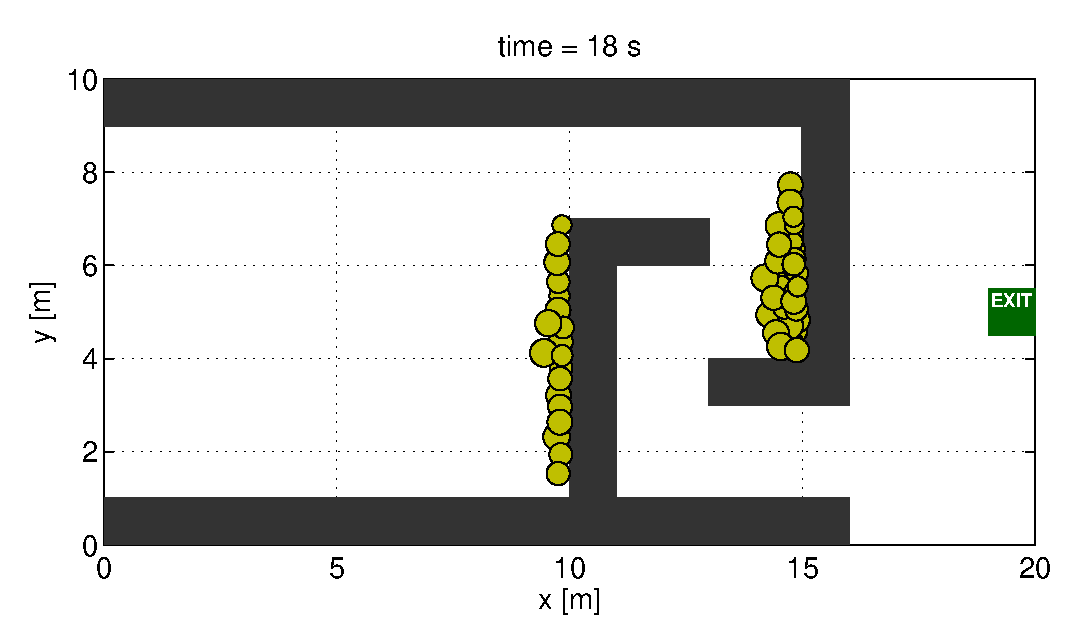
\includegraphics[width=0.7\textwidth]
	{figures/Model2_direct_1_001800.eps}
	\caption{Model with direct exit force formulation for a pedestrian flow around complicated architecture. (a) Initial setup, (b) agents arriving at the barrier walls and accumulating and (c) agents getting stucked and not able to move around an obstacle at the end of the simulation.}
	\label{fig:simple3}
	\end{center}
\end{figure}

The walls are placed in a way that the pedestrians have to move around corners and even away from the exit to finally arrive there. This is not straight forward and a simple exit force formulation is not able to describe the pedestrian flow in such a case (Fig.~\ref{fig:simple3}). The Agents get captured by obstacles with no direct passage towards the exit and are not able to leave such a place. 

The more elaborated shortest path formulation, on the other hand, can describe such a more complicated pedestrian flow in a realistic manner (Fig.~\ref{fig:simple4}). The agents are able to see all possible passages towards an exit in the whole model and are therefore able to chose the fastest way.

\begin{figure}
	\begin{center}
	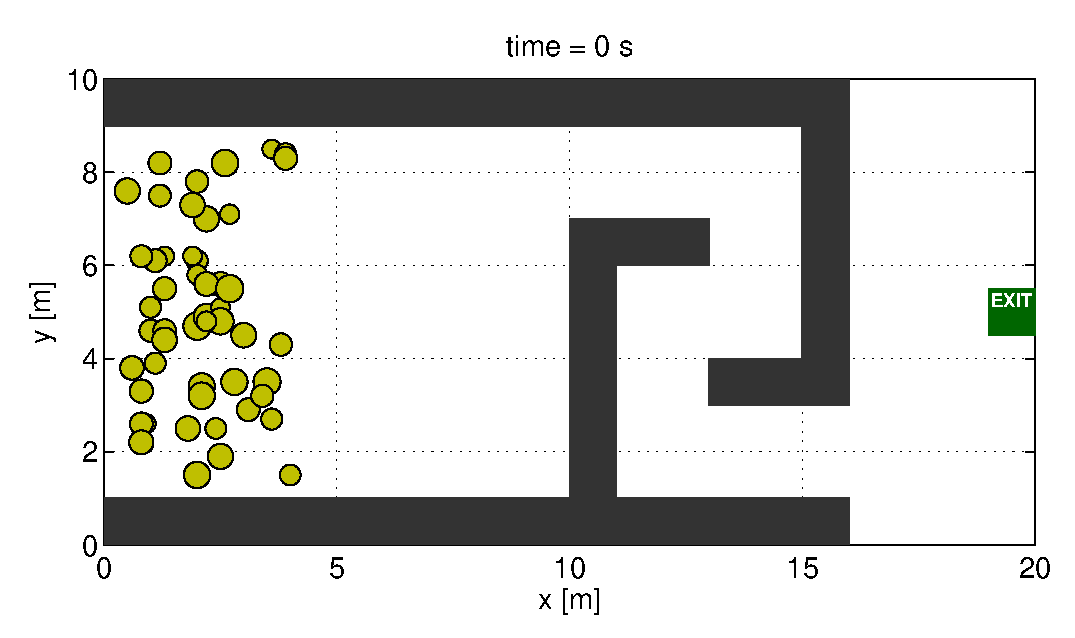
\includegraphics[width=0.7\textwidth]
	{figures/Model2_fastest_1_000000.eps}
	\qquad
	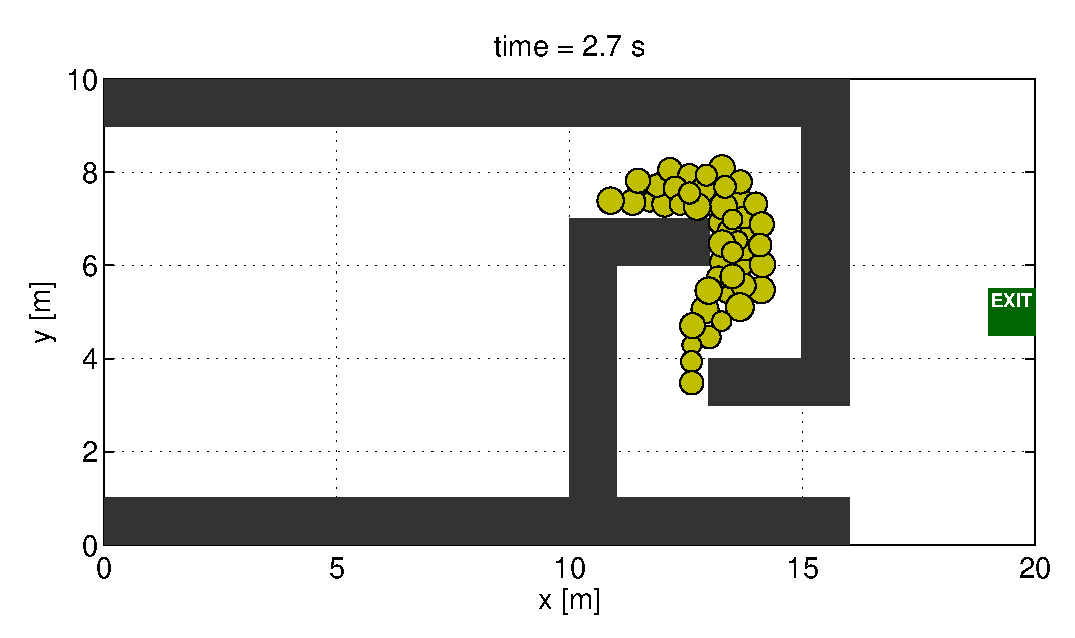
\includegraphics[width=0.7\textwidth]
	{figures/Model2_fastest_1_000270.eps}
	\qquad
	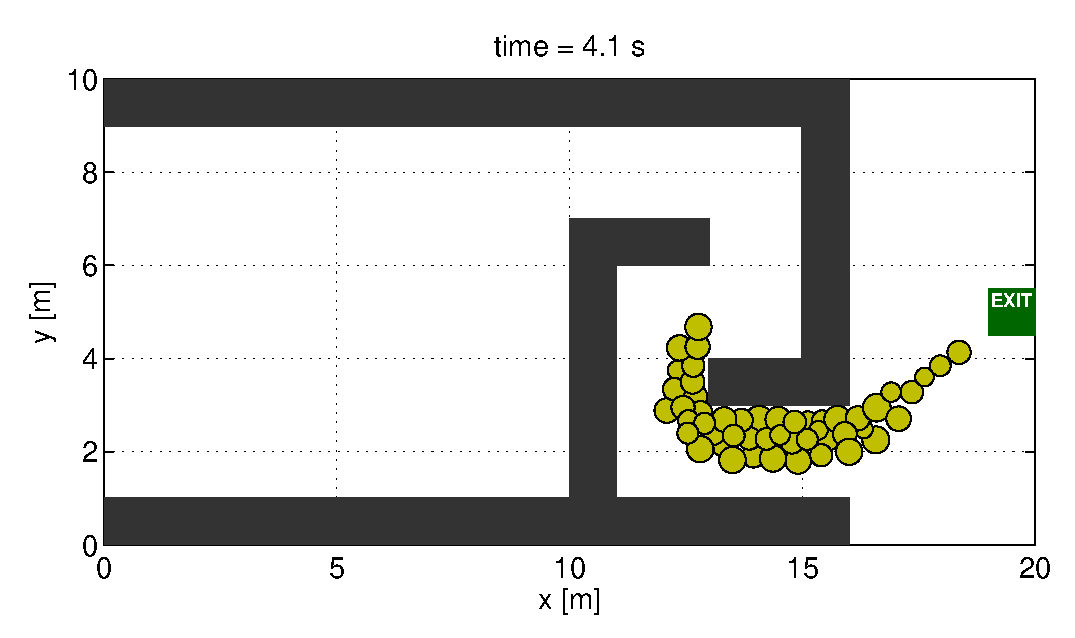
\includegraphics[width=0.7\textwidth]
	{figures/Model2_fastest_1_000410.eps}
	\caption{Model including shortest path formulation for a pedestrian flow around complicated architecture. (a) Initial setup, (b) agents moving closely around corners and (c) agents able to move around obstacles in the fastest way and arriving the exit at the end of the simulation.}
	\label{fig:simple4}
	\end{center}
\end{figure}

\subsection{Simple evacuation bottleneck: One exit with topography}
\subsection{Simple evacuation bottleneck: Two exits}
\subsection{Evacuation through a road network}
\subsection{Evacuation through a road network with topography and flooding}
\subsection{Evacuation of a beach in the case of a tsunami event}

\section{Summary and Outlook}

Christmas Tree!

\section{References}

- Helbing 2000




\end{document}  


%\begin{figure}
%	\begin{center}
%	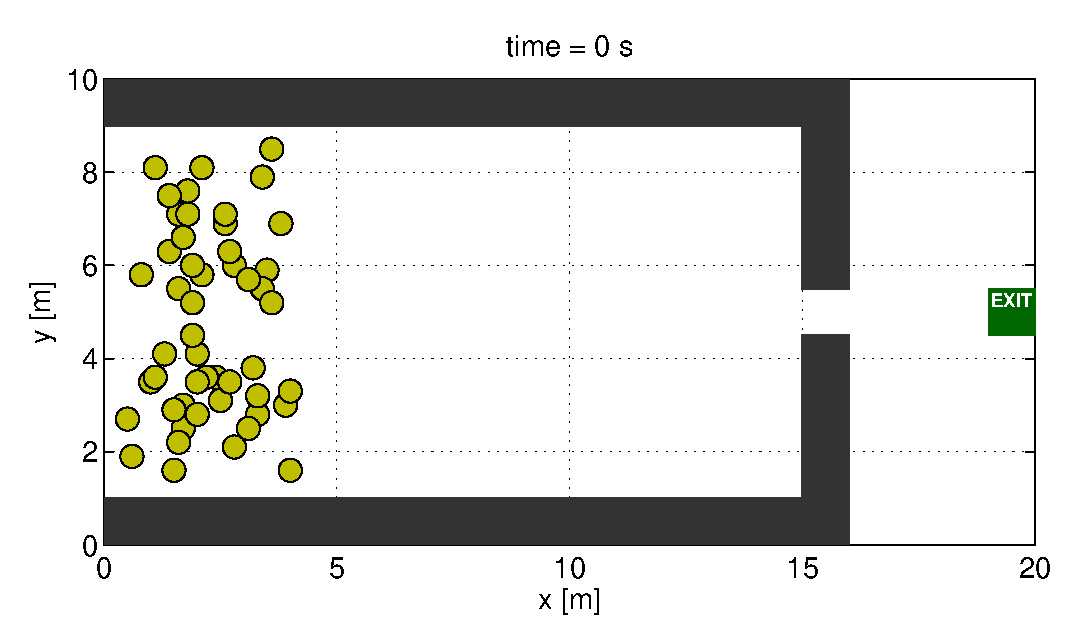
\includegraphics[width=16cm]{figures/Model1_direct_1_000000.eps}
%	\caption{Simple simulation of an evacuation bottleneck. Agents (yellow) try to exit a room surrounded by repulsive walls (red) with an 1 m-wide door towards an attractive exit (green).}
%	\label{fig:simple0}
%	\end{center}
%\end{figure}
%
%\begin{figure}
%	\begin{center}
%	\includegraphics[width=1.0\textwidth]
%	{figures/Model1_direct_1_000000.eps}
%	\qquad
%	\includegraphics[width=1.0\textwidth]
%	{figures/Model1_direct_1_000000.eps}
%	\caption{caption}
%	\label{fig:simple1}
%	\end{center}
%\end{figure}

 
